\documentclass[12pt,a4paper,oneside]{article}
\usepackage[dutch]{babel}
\usepackage{graphicx}
\usepackage{amsmath}
\usepackage{listings}
\usepackage[justification=centering]{caption}
\usepackage{epstopdf}
\usepackage{color} %red, green, blue, yellow, cyan, magenta, black, white
\definecolor{mygreen}{RGB}{28,172,0} % color values Red, Green, Blue
\definecolor{mylilas}{RGB}{170,55,241}


\newcommand{\todo}[1]{\textcolor{red}{TODO: #1}\PackageWarning{TODO:}{#1!}}

% No tab at start of paragraph
\setlength{\parindent}{0em}
\setlength{\parskip}{1em}
\begin{document}

\lstset{language=Matlab,%
    %basicstyle=\color{red},
    breaklines=true,%
    morekeywords={matlab2tikz},
    keywordstyle=\color{blue},%
    morekeywords=[2]{1}, keywordstyle=[2]{\color{black}},
    identifierstyle=\color{black},%
    stringstyle=\color{mylilas},
    commentstyle=\color{mygreen},%
    showstringspaces=false,%without this there will be a symbol in the places where there is a space
    numbers=left,%
    numberstyle={\tiny \color{black}},% size of the numbers
    numbersep=9pt, % this defines how far the numbers are from the text
    frame=single, % adds a frame around the code
    emph=[1]{for,end,break},emphstyle=[1]\color{red}, %some words to emphasise
    %emph=[2]{word1,word2}, emphstyle=[2]{style},    
}


\title{Information Theory: \\ Project : Distributed Storage}
\author{Fr\'ed\'erique De Baerdemaeker, Caroline De Brouwer and\\Titouan Vervack}
\maketitle

\section{Data storage}
\subsubsection*{Question 1}
% It is generally considered that RAID 5 systems are not suitable for larger
% disk sizes. Explain why. Is the same true for RAID 6?
% http://www.enterprisestorageguide.com/raid-disk-rebuild-times
% http://www.zdnet.com/article/why-raid-5-stops-working-in-2009/
There are 2 reasons RAID 5 is not considered suitable for larger disk sizes: time and unrecoverable read errors. The time issue is not directly correlated to RAID 6, but to RAID in general. 

When a disk fails, the entire disk will be rebuilt. Because it's the entire disk being rebuilt, there is a best-case duration of the disk size divided by the sequential write speed. On top of this there is also always the parity calculation that has to be done to rebuild redundancy, which also brings some overhead. Because this scales directly with the disk size, larger disks will have a huge impact on the time it takes to rebuild one.

The second problem is correlated to the first one, when a rebuild happens, the whole disk's worth of data needs to be read of the remaining disks in the array. Because this is a lot of work, there is a much higher chance a second disk failure will occur. Again, larger disk size means more data needs to be more read, means higher chance of failure. A second disk failure during the first one's rebuilding means there will be data loss in RAID 5.

RAID 6 does a better job at solving these problems, but only for current disk sizes. We now have 2 disks we can read from to reconstruct the data (double parity) which speeds up rebuilding and allows to actually withstand 2 simultaneous disk failures. But when the disk sizes increase again, there is again a larger chance for disk failures occur and so the chance a third disk will fail also grows. And as with RAID 5, RAID 6 will have data loss with 3 disk failures. The root of these issues lies in the increasing capacity of disks and the steady rate for read errors, so ultimately these kind of RAID configurations will always struggle with increasing disk sizes.

\subsubsection*{Question 2}
``Nested RAID levels, also known as hybrid RAID, combine two or more of the standard RAID levels to gain performance, additional redundancy or both, as a result of combining properties of different standard RAID layouts.'' - Wikipedia
\\\\
Standard RAID has 10 levels (0 through 9), they describe the configuration of an array of disks and the patterns how the data is written to the disks. These properties determine the fault tolerance and space efficiency of the array. The RAID level also has a minimum amount of drives, for the standard levels it varies between 1 to 4 drives.

When we nest RAID levels, we combine 2 levels to gain advantages from both levels.
We can illustrate by taking a look at RAID 60 which combines RAID 6 (Double Parity) and RAID 0 (Stripe). RAID 0 is a very basic configuration where the data is split across drives (striping), meaning it can be used with a minimum of 2 drives. This allows for a big increase in performance, but if any drive fails, there will be data loss. This set-up does not protect and makes you more vulnerable to failures.
RAID 6 also uses striping, but also has double parity which is distributed among the drives. Double parity means that for each data element there are 2 parity blocks distributed among the drives. Because the double parity, write and read performance take a hit, but it allows recovery from a fault and a disk failure. This set up does require a minimum of 4 drives (2 data, 2 parity).

RAID 60 combines these 2 by having multiple RAID 6 arrays (of 4 disks) and striping these (RAID 0). This means it has the data striped over 2 different RAID 6 arrays, and each of those arrays has 2 parity blocks for the data distributed over the drives. RAID 60 requires a minimum 8 disks and can handle up to two disk failures for each RAID 6 sub-array. So for a 2x4 disk set-up, it can tolerate up to 4 disk failures.

\subsubsection*{Question 3}
The data concerning reliability for both drives can be found below:
\begin{table}[h]
\centering
\begin{tabular}{l|c|c}
                                          & WD Xe                    & Seagate Kinetic \\\hline
(Un)load cycles                           & 600.000                  & 300.000         \\
Non-recoverable read errors per bits read & \textless 1 in $10^{16}$ & 1 in $10^{14}$  \\
MTBF (hours)                              & 2.000.000                & 800.000         \\
\end{tabular}
\end{table}
The WD Xe drive is the better drive out of the two when considering these statistics, it scores better for all 3 statistics. Thus I would choose for the WD Xe.\par
We now compute the AFR for both drives using the formula:\\
\begin{equation*}
\centering
AFR = \frac{1}{MBTF/8760} * 100
\end{equation*}
The AFR for both drives can be found below:
\begin{table}[h]
\centering
\begin{tabular}{l|c|c}
    & WD Xe     & Seagate Kinetic \\\hline
AFR & $0,438\%$ & $1,095\%$       \\
\end{tabular}
\end{table}
\subsubsection*{Question 4}
Object storage is a term that refers to the storing of data as objects rather than files. They aren't stored in a hierarchy like in a file system but in a flat object space. Objects contain metadata for identification. It is possible to have an object storage system where objects have different levels of data protection. To protect the data, object based storage devices often use erasure codes. To protect the data against disk failures, objects can also be replicated across multiple servers and locations.

\section{Reed Solomon Coding}
\subsubsection*{Encoding}
All calculations of this part can be found in the file \verb|ReedSolomon.m|
\begin{itemize}
	\item To show that p(D) is a primitive polynomial we prove that $\alpha^k$ is 1 if and only if $k=255$. 
	\lstinputlisting[language=Matlab, firstline=6, lastline=16]{../ReedSolomon.m}
	\item The generator polynomial of a Reed-Solomon code is constructed as follows: \\
		\begin{equation*}
			g(x) = (X-\alpha^1)(X-\alpha^2)...(X-\alpha^{2*t})
		\end{equation*}
		In this case, t=3 so we can calculate the polynomial using the following Matlab code:
		\lstinputlisting[language=Matlab, firstline=20, lastline=22]{../ReedSolomon.m}
		The resulting generator polynomial is
		\begin{equation*}
			g(x) = x^6 + 126x^5 + 4x^4 + 158x^3 + 58x^2 + 49x + 117
		\end{equation*}
	\item The check polynomial is calculated the same way, but the instead of taking alpha to the powers of 1 to $2*t$ we take the ones from $2*t+1$ to $q-1$ with $q$ being $2^8$ or $256$. 
	This generator polynomial is huge to type out so we refer to the output of the Matlab file for the coefficients. As a check, if we take the convolution of $g(x)$ and $h(x)$ we get $x^n -1$ so we know the generator and check polynomials are correct.
	\item We can calculate the code by calculating $c'(x)$: $c'(x) = b(x)G(x)$ where $b(x) = (b^{(1)}(x),b^{(2)}(x),...,b^{(k)}(x))$ and $c'(x) = c^{(1)}(x),c^{(2)}(x),...,c^{(n)}(x)$. Applying parallel-to-serial conversion now yields the code as follows: $c(x) = c^{(1)}(x^n),xc^{(2)}(x^n),...x^{n-1}c^{(n)}(x^n)$.\\
	This means that every node has to execute a multiplication of a generator polynomial with $b(x)$. Thus every node will now have a calculated a polynomial $c^{(i)}(x)$ where $i \in [1,n]$. The nodes then have to multiply $c^{(i)}(x)$ with $x^{i-1}$. Once this is done, they send their new polynomial to a central node which will add all of these polynomials together to generate $c(x)$.
	\item In MDS codes, the minimal Hamming distance $d$ satisfies the equation $k + d = n + 1$ (Singleton bound). This means that the minimal Hamming distance in this case is $7$.
	\item A Reed-Solomon code only needs $2t$ parity symbols to correct $t$ errors. Also, because it is not binary, but uses multiple bits for one symbol, it is possible that a burst of bit errors still only counts as one symbol error, which makes an RS code more robust.
	
\subsection*{Erasure and error decoding}
    \item The symbol error correcting capability of a BCH code (and thus an RS code) is t. A symbol error can range from 1 bit error to m bit errors (where m is the size of a symbol). The minimum bit errors we can recover is 1, this is when there is 1 bitrot in 1 symbol. As $t = 3$ and $m = 8$ the maximum bitrots that can be recovered is $3 * 8 = 24$.\par
    \item We were not able to implement the selfHeal method correctly. We have searched through the course as well as various papers and documentation on error correcting with Reed Solomon codes and we have tried to implement the Berlekamp-Massey algorithm to find the error locating polynomial (in the function \verb|findErrorPolynomial()|). For finding the roots of this polynomial we have implemented Chien search. We suspect something goes wrong in the Berlekamp-Massey method.
    \item Because we couldn't get the selfHeal method correct, we also couldn't simulate correct bit error values.
    \item According to the study performed by CERN, $1.32*10^{-9}$\% of the of the total data got corrupted after six months. If we apply this to an entire year and only 36 petabyte of data we get that there are 95.010.310 corrupted bytes or about 95 megabytes.
    \begin{equation*}
        \centering
        1.32*10^{-9} * 2 * 36 * 10^{15} = 95010310
    \end{equation*}
If we assume the errors are equally divided, RS encoding will be able to repair all errors as only one byte at a time would fail, our symbols are 1 byte long and we are able to correct up to 3 symbols at once. Even if the errors are not equally divided, the chance that four succeeding symbols get corrupted is very small, thus almost no errors should slip past. From this analysis we can conclude that bitrot is not a big problem.


\section{Locally Repairable Codes}
    \item Since $k = 2$ and $r = 5$, we get that $K = 6$. With these values, we can now give the table representing the data stored in the second repair group of the LRC code:
\begin{table}[h]
\centering
\begin{tabular}{l|c|c|c|c|c|c}
                  & node 1       & node 2       & node 3       & node 4       & node 5       & node 6\\\hline
blocks of $c^{1}$ & \textcolor{red}{$c^{1}_{7}$}  & $c^{1}_{8}$  & $c^{1}_{9}$  & $c^{1}_{10}$ & $c^{1}_{11}$ & $c^{1}_{12}$\\
blocks of $c^{2}$ & $c^{2}_{8}$  & $c^{2}_{9}$  & $c^{2}_{10}$ & $c^{2}_{11}$ & $c^{2}_{12}$ & $c^{2}_{7}$\\
blocks of $c^{3}$ & $c^{3}_{9}$  & $c^{3}_{10}$ & $c^{3}_{11}$ & $c^{3}_{12}$ & \textcolor{red}{$c^{3}_{7}$}  & $c^{3}_{8}$\\
blocks of $c^{4}$ & $c^{4}_{10}$ & $c^{4}_{11}$ & $c^{4}_{12}$ & \textcolor{red}{$c^{4}_{7}$}  & $c^{4}_{8}$  & $c^{4}_{9}$\\
blocks of $c^{5}$ & $c^{5}_{11}$ & $c^{5}_{12}$ & \textcolor{red}{$c^{5}_{7}$}  & $c^{5}_{8}$  & $c^{5}_{9}$  & $c^{5}_{10}$\\
blocks of s       & $s_{12}$     & \textcolor{red}{$s_{7}$}      & $s_{8}$      & $s_{9}$      & $s_{10}$     & $s_{11}$
\end{tabular}
\end{table}\\
    \item The elements required to recover $c^{(2)}_{K + 1} = c^{(2)}_{7}$ have been highlighted in red in the previous table. To recover this error we do the following. First, we calculate the syndrom $s'$ which does not take the codeword we're trying to recover into account:
    \begin{equation}
        \centering
        s_j' = \sum^r_{\substack{i = 1\\i \neq i'}} c^i_j
    \end{equation}
    Here $i'$ is the i of the code word we're trying to recover. From this new syndrom and the old syndrom and knowing that the calculation of these syndroms is just a XOR of the codewords, we can now recover the corrupted codeword:\\
        \begin{center}
        $c^{(i')}_j = s_j \oplus s_j'$\\
        \end{center}
    In this formula $c^{(i')}_j$ represents the corrupted code word.
    As we didn't use $c^{(i)}_j$ in our new syndrom we know that $c^{(i)}_j$ is the difference between the two syndroms.\par
    
    \item For our own code we use the same table as before but we add a new parity bit. We will call it t, t can be calculated as follows:
    \begin{equation*}
        \centering
        t = [t_1,...,t_n] = \sum^{r}_{i = 1}c^{(i)} >> (i - 1)
    \end{equation*}
    Where $>>$ is the circular right bit shift.\\
    The table will look as follows:\\
    \begin{table}[h]
\centering
\begin{tabular}{l|c|c|c|c|c|c}
                  & node 1       & node 2       & node 3       & node 4       & node 5       & node 6\\\hline
blocks of $c^{1}$ & $c^{1}_{7}$  & $c^{1}_{8}$  & $c^{1}_{9}$  & $c^{1}_{10}$ & $c^{1}_{11}$ & $c^{1}_{12}$\\
blocks of $c^{2}$ & $c^{2}_{8}$  & $c^{2}_{9}$  & $c^{2}_{10}$ & $c^{2}_{11}$ & $c^{2}_{12}$ & $c^{2}_{7}$ \\
blocks of $c^{3}$ & $c^{3}_{9}$  & $c^{3}_{10}$ & $c^{3}_{11}$ & $c^{3}_{12}$ & $c^{3}_{7}$  & $c^{3}_{8}$ \\
blocks of $c^{4}$ & $c^{4}_{10}$ & $c^{4}_{11}$ & $c^{4}_{12}$ & $c^{4}_{7}$  & $c^{4}_{8}$  & $c^{4}_{9}$ \\
blocks of $c^{5}$ & $c^{5}_{11}$ & $c^{5}_{12}$ & $c^{5}_{7}$  & $c^{5}_{8}$  & $c^{5}_{9}$  & $c^{5}_{10}$\\
blocks of s       & $s_{12}$     & $s_{7}$      & $s_{8}$      & $s_{9}$      & $s_{10}$     & $s_{11}$    \\
blocks of t       & $t_{1}$      & $t_{2}$      & $t_{3}$      & $t_{4}$      & $t_{5}$      & $t_{6}$
\end{tabular}
\end{table}\\
One failed node can be repaired in the same way as before, we just ignore the t.\\
Two failed nodes can be recovered with the help of t. If the 2 errors occur in the codewords needed to calculate s, we use t to recover one of these errors and then use s to recover the other one. To recover using t we use the same methodology as when we recover 1 erasure with s. If both errors occur in the codewords needed to calculate t, we use s to recover one of these errors and then we use t to recover the other one. All the errors can always be solved by first recovering one with t and the other with s.\\
\item The higher the repair locality r, the higher the actual storage capacity. Thus having more repair nodes is beneficial to the amount of storage we can actually use.\\
The plot has been generated using \verb|RS_LRC_own_plot.m|. You can find it below:
\begin{figure}
\centering
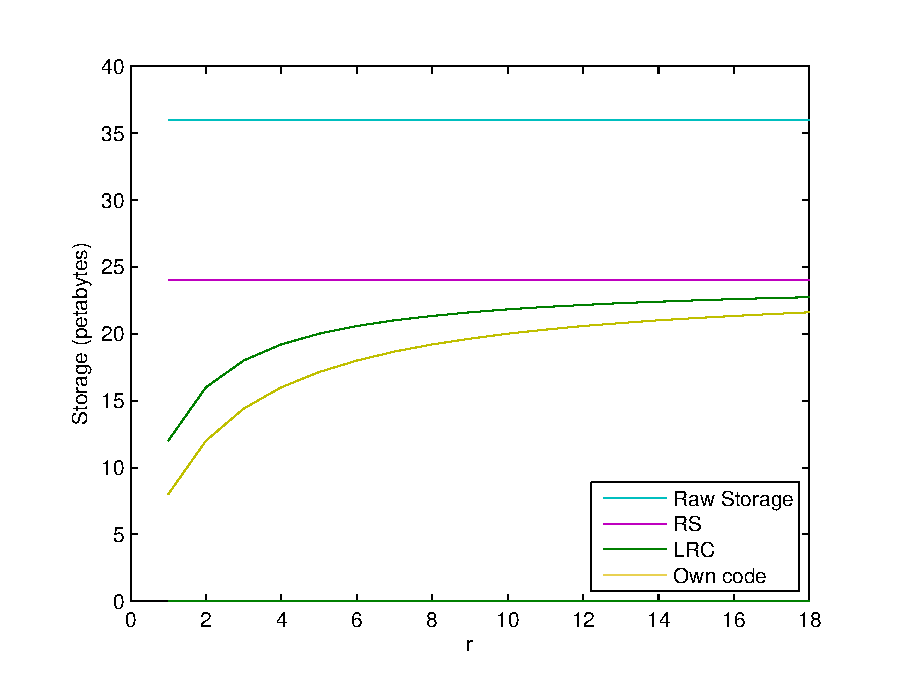
\includegraphics{RS_LRC_own_plot.eps}
\end{figure}
\end{itemize}
\end{document}

